\subsection{The \textit{broadcast-and-then-aggregate} operation}

We consider a generalized \textit{broadcast-and-then-aggregate} operation that has the following standard form:
\lstset{
  frame=lrtb,
  backgroundcolor=\color{aliceblue},
  numbers=left,
  numbersep=1em,
  xleftmargin=1em,
  linewidth=\linewidth
}
\begin{lstlisting}[language=code_example, caption={}]
function (:$\textit{BroadcastAndThenAggregate}\ (f::(\alpha \rightarrow \gamma \rightarrow \beta), c::\gamma, \oplus::(\beta\rightarrow\theta\rightarrow \theta),\ s_0::\theta,\ xs::[\alpha])$:)  
  (:$s = s_0$:)  // initialize the accumulator
  foreach((:$x$:) in (:$xs$:))
    (:$s = \oplus(s, f(x, c))$:)  // broadcast c and accumulate s
  return (:s:)
\end{lstlisting}

The \textit{broadcast-and-then-aggregate} operation is defined by the quadruple $R=<f, c, \oplus, s_0>$.
$f$ is a function of type $\alpha \rightarrow \gamma \rightarrow \beta$, $c$ is a constant value of type $\gamma$,
$\oplus$ is a binary operator of type $\beta \rightarrow \theta \rightarrow \theta$. $s$ is an accumulator of type $\theta$ that store the aggregated value, and are initialized to $s_0$.

The computational process proceeds by enumerating each input value $x$ from the input list $xs$,
broadcasting $c$ to $x$ by applying $y=f(x, c)$, and then aggregating $s$ according to $s = s \oplus y$.
It is important to note that \textit{there is no communication among the evaluations of $f(x,c)$}.

We can use the diagram below to visualize this operation.

\begin{figure}[h]
  \centering
  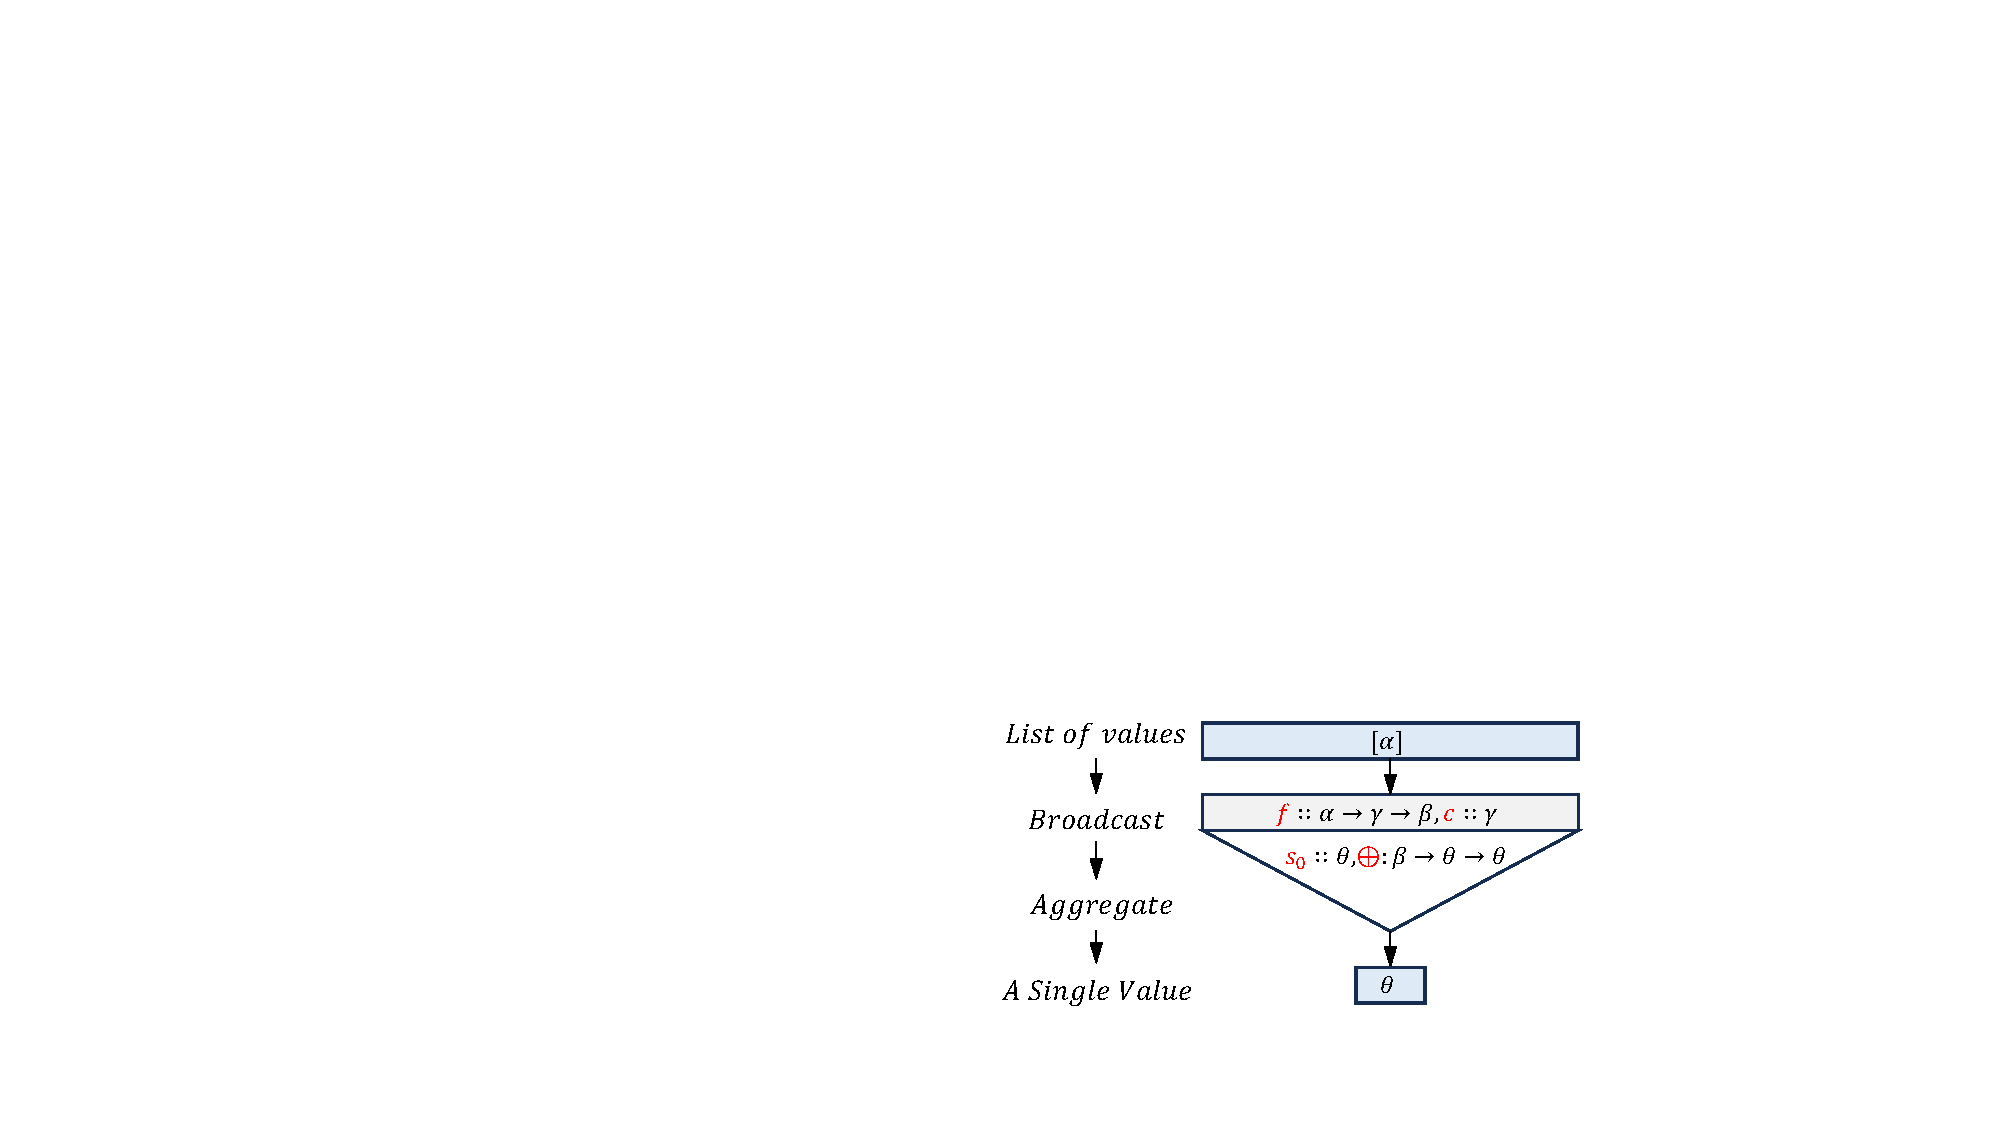
\includegraphics[width=0.4\textwidth]{figures/map_and_aggregate.pdf}
  \caption{The diagram to visualize the \textit{broadcast-and-then-aggregate} operation.}
\end{figure}

\subsection{The running example: attention in \textit{Broadcast-and-then-Aggregate}}

\textcolor{red}{Neural network computations can be expressed uniformly as a dataflow graph of broadcast-and-then-aggregate operations}.
As a concrete example, we can express attention using a set of {broadcast-and-then-aggregate} operatiosn. Figure \ref{attn} shows the corresponding dataflow graph.

\begin{equation}
\text{Attn(Q, K, V)}=\text{softmax}(QK^T)V \label{eq::attn}
\end{equation}

\begin{figure}[h]
  \centering
  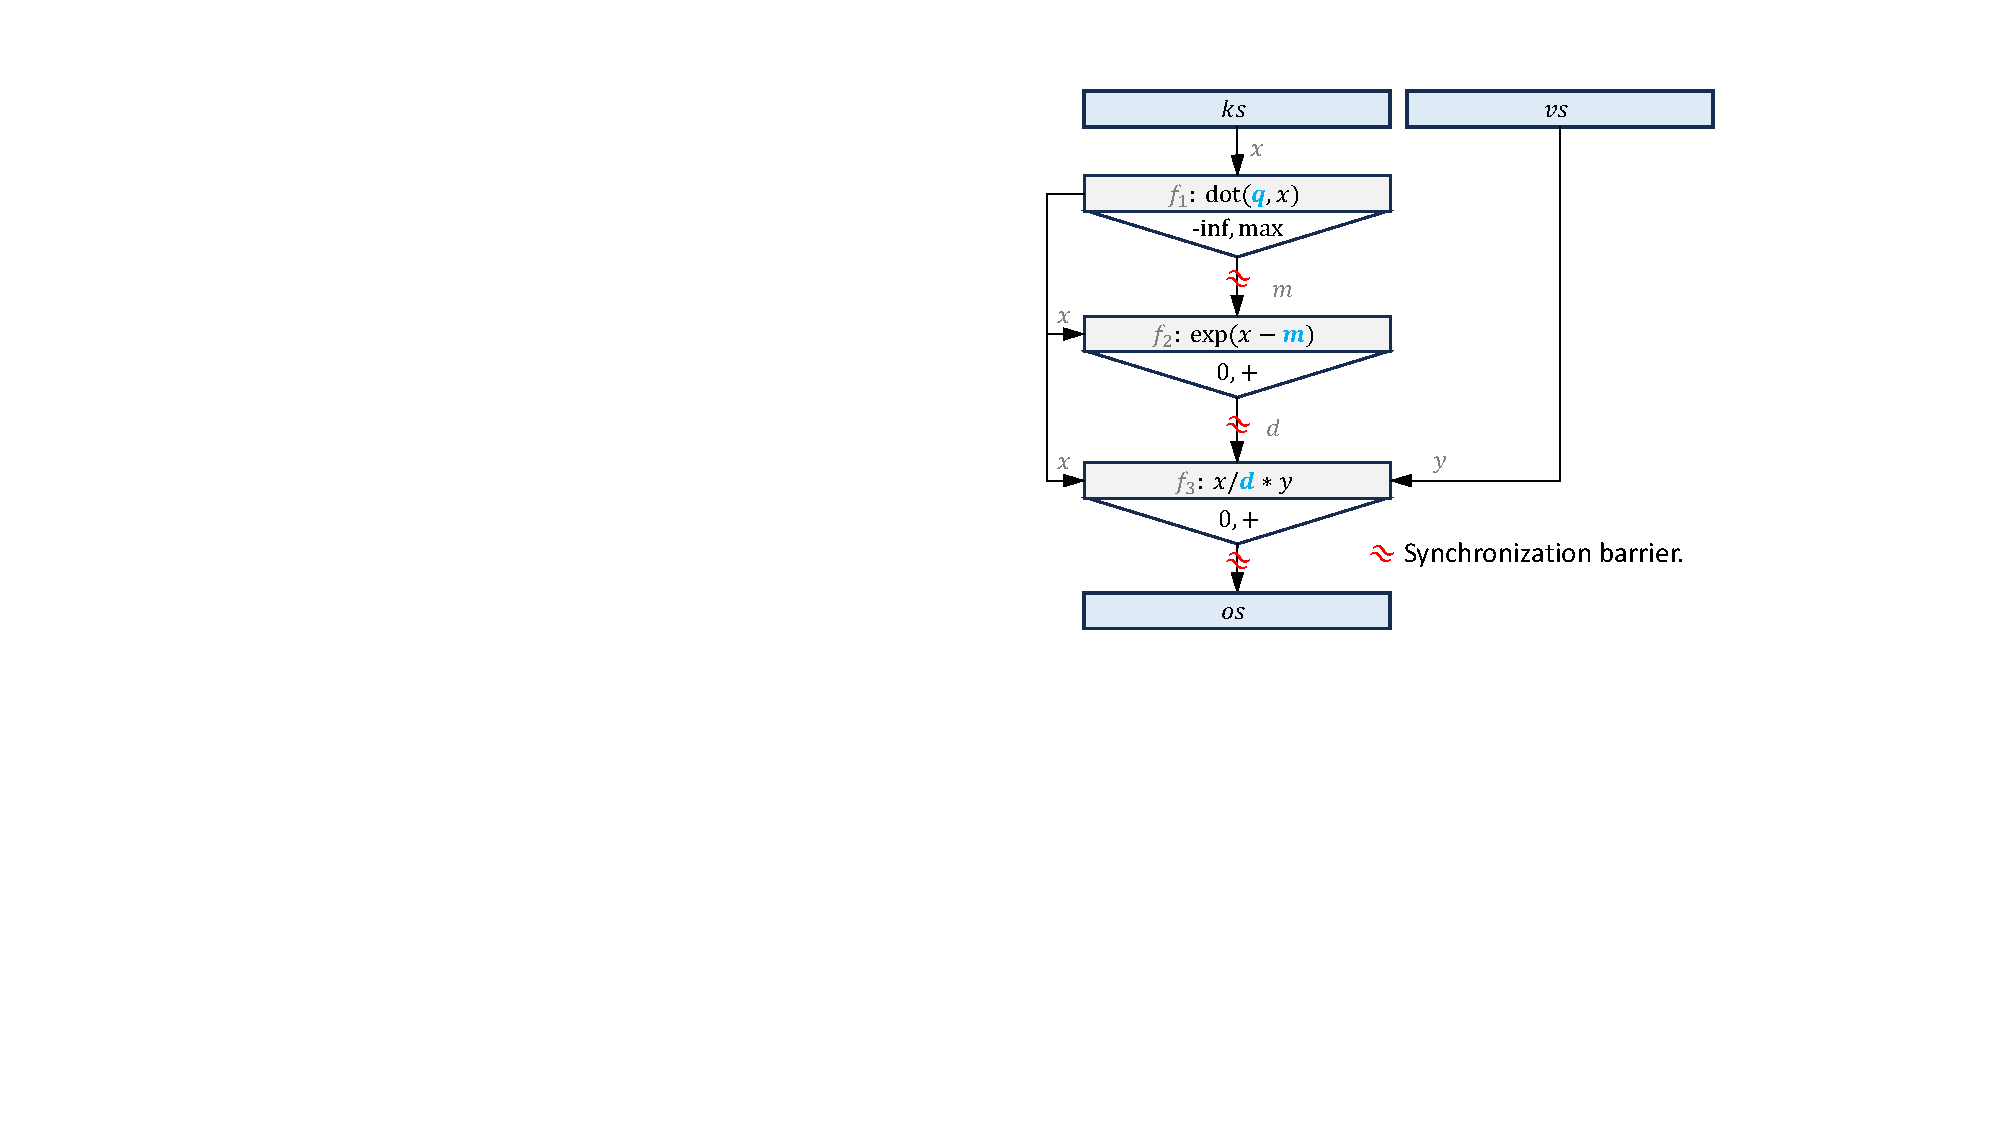
\includegraphics[width=0.5\textwidth]{figures/attention_expression_tree1.pdf}
  \caption{Express attention function using \textit{broadcast-and-then-aggregate}.}\label{attn}
\end{figure}